\section{Rare Disease Forecasting}

One of the key event classes studied in EMBERS included forecasting outbreaks of $4$ rare diseases (hantavirus, cholera, yellow fever and machupo) in 10 countries of Latin America. EMBERS rare disease model employed a corpus of publicly available health-related news articles from HealthMap (cite) to forecast discrete incidences of rare diseases. Similar to ILI, rare disease model was also tuned over time to incorporate our findings over time. Over the course of our project, the forecasts generated by the EMBERS rare disease model were compared against the forecasts generated by a base rate model. The base rate model generates forecasts for a particular month in future based on the average frequency of rare disease incidences reported over a past time window of 3 months.


\subsubsection{Successful forecasts}

EMBERS rare disease model successfully forecasted the hantavirus outbreaks in Chile and Argentina during 2013 and 2014. EMBERS model was also able to forecast successfully the rate changes in hantavirus incidences in Argentina during 2013. However, since the base rate model generated forecasts based only on the past frequency of incidences, the base rate model detected the rate changes in hantavirus incidences with a certain delay in comparison to the EMBERS model. 

\begin{figure}
  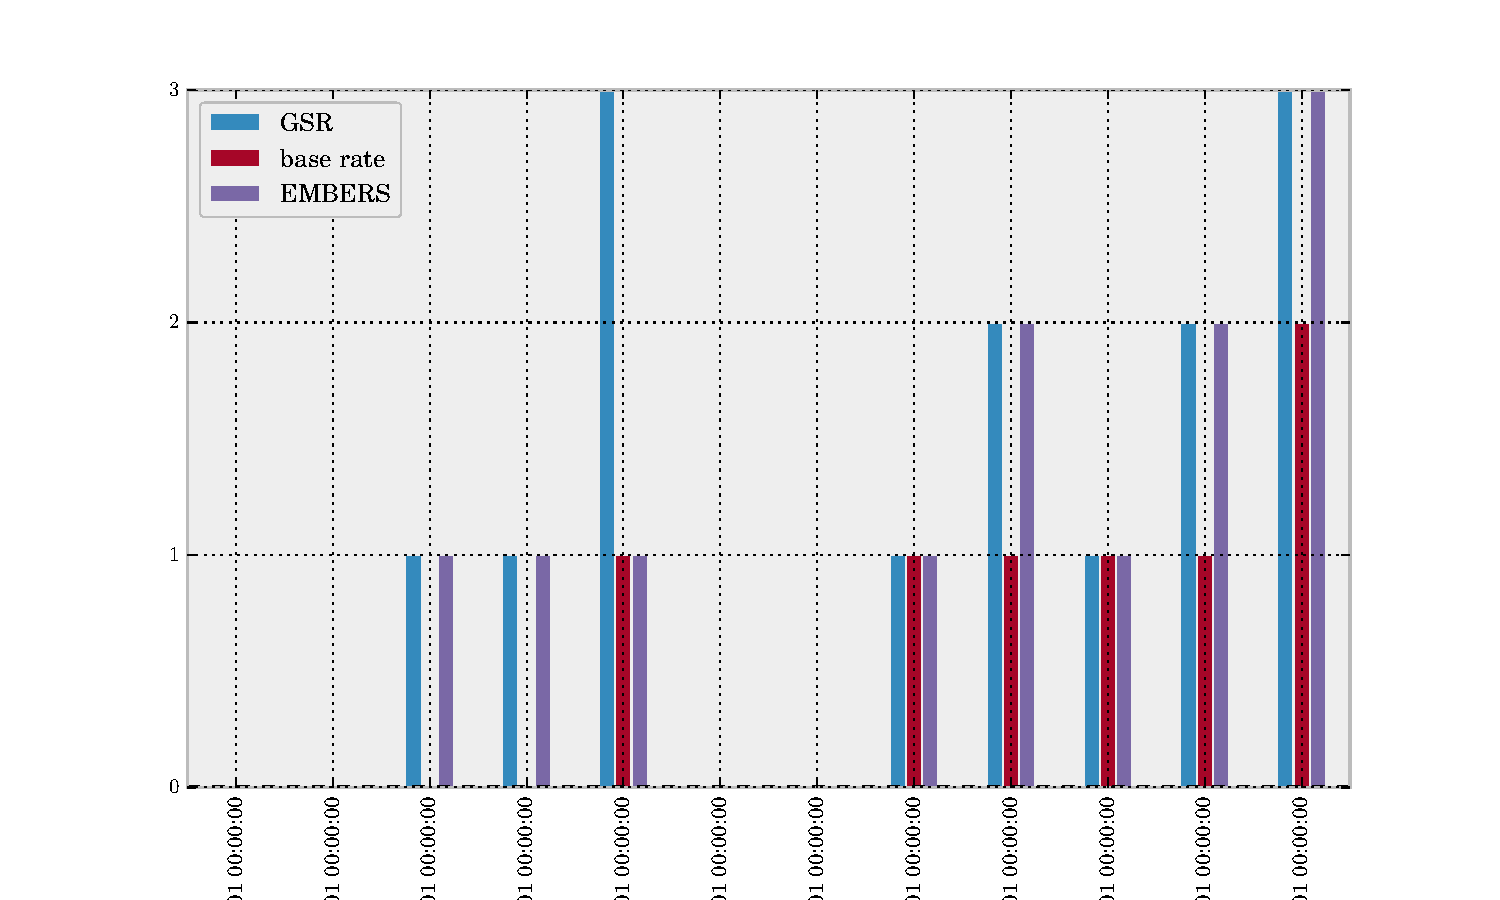
\includegraphics[width=0.4\textwidth]{../figures/ili/embers_vs_baserate}
  \caption{\label{fig:embers_vs_baserate} Bar plot showing the number of hantavirus incidences recorded in GSR (blue), number of GSR incidences successfully forecasted by the EMBERS model (red) and number of GSR incidences successfully forecasted by the base rate model (green) for Argentina during each month in 2013.}
\end{figure}

In Figure~\ref{fig:embers_vs_baserate}, we see that the base rate model takes 2 months later than EMBERS to capture the uptick in Hantavirus incidences at the end of 2012-2013 season. The base rate model also takes 3 months later than EMBERS to detect the uptick in Hantavirus incidences at the start of 2013-2014 season. 


\subsubsection{Failures}

EMBERS rare disease model failed to forecast the cholera outbreak in Mexico during the months of October and November 2013. One of the possible reasons is that this cholera outbreak spread to Mexico from its neighboring country Cuba as shown in Figure~\ref{fig:cholera_mexico}. Therefore, there was no prior signal about this outbreak in the HealthMap corpus. Alternative data sources, such as travel patterns could have helped us in forecasting this outbreak.

\begin{figure}
  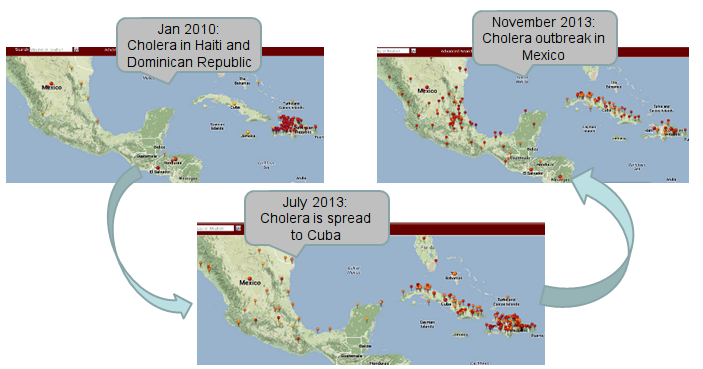
\includegraphics[width=0.4\textwidth]{../figures/ili/cholera_mexico}
  \caption{\label{fig:cholera_mexico} Spread of cholera from Haiti and Dominican Republic to Cuba and finally to Mexico.}
\end{figure}
